
\documentclass[ 
	% -- opções da classe memoir --
	article,			% indica que é um artigo acadêmico
	11pt,				% tamanho da fonte
	oneside,			% para impressão apenas no verso. Oposto a twoside
	a4paper,			% tamanho do papel. 
	% -- opções da classe abntex2 --
	%chapter=TITLE,		% títulos de capítulos convertidos em letras maiúsculas
	%section=TITLE,		% títulos de seções convertidos em letras maiúsculas
	%subsection=TITLE,	% títulos de subseções convertidos em letras maiúsculas
	%subsubsection=TITLE % títulos de subsubseções convertidos em letras maiúsculas
	% -- opções do pacote babel --
	english,			% idioma adicional para hifenização
	brazil,				% o último idioma é o principal do documento
	]{abntex2}


% --- 
% PACOTES
% ---

% ---
% Pacotes fundamentais 
% ---
\usepackage{cmap}				% Mapear caracteres especiais no PDF
\usepackage{lmodern}			% Usa a fonte Latin Modern
\usepackage[T1]{fontenc}		% Selecao de codigos de fonte.
\usepackage[utf8]{inputenc}		% Codificacao do documento (conversão automática dos acentos)
\usepackage{indentfirst}		% Indenta o primeiro parágrafo de cada seção.
\usepackage{nomencl} 			% Lista de simbolos
\usepackage{color}				% Controle das cores
\usepackage{graphicx}			% Inclusão de gráficos
\usepackage{csvsimple}
\usepackage{epstopdf}
\usepackage{multirow}
%\usepackage[nolists,tablesfirst]{endfloat}
% ---
		
% ---
% Pacotes adicionais, usados apenas no âmbito do Modelo Canônico do abnteX2
% ---
\usepackage{lipsum}				% para geração de dummy text
% ---
		
% ---
% Pacotes de citações
% ---
\usepackage[brazilian,hyperpageref]{backref}	 % Paginas com as citações na bibl
\usepackage[alf]{abntex2cite}	% Citações padrão ABNT
% ---

% ---
% Configurações do pacote backref
% Usado sem a opção hyperpageref de backref
\renewcommand{\backrefpagesname}{Citado na(s) página(s):~}
% Texto padrão antes do número das páginas
\renewcommand{\backref}{}
% Define os textos da citação
\renewcommand*{\backrefalt}[4]{
	\ifcase #1 %
		Nenhuma citação no texto.%
	\or
		Citado na página #2.%
	\else
		Citado #1 vezes nas páginas #2.%
	\fi}%
% ---

% ---
% Informações de dados para CAPA e FOLHA DE ROSTO
% ---
\titulo{Relatório de atividades: Uso do classificador Bayesiano} 
\autor{David Clifte\thanks{cliftedavid@gmail.com}}
\local{Brasil}
\data{2015, v-1.0}
% ---

% ---
% Configurações de aparência do PDF final

% alterando o aspecto da cor azul
\definecolor{blue}{RGB}{41,5,195}

% informações do PDF
\makeatletter
\hypersetup{
     	%pagebackref=true,
		pdftitle={\@title}, 
		pdfauthor={\@author},
    	pdfsubject={Modelo de artigo científico com abnTeX2},
	    pdfcreator={LaTeX with abnTeX2},
		pdfkeywords={abnt}{latex}{abntex}{abntex2}{atigo científico}, 
		colorlinks=true,       		% false: boxed links; true: colored links
    	linkcolor=blue,          	% color of internal links
    	citecolor=blue,        		% color of links to bibliography
    	filecolor=magenta,      		% color of file links
		urlcolor=blue,
		bookmarksdepth=4
}
\makeatother
% --- 

% ---
% compila o indice
% ---
\makeindex
% ---

% ---
% Altera as margens padrões
% ---
\setlrmarginsandblock{4cm}{4cm}{*}
\setulmarginsandblock{4cm}{4cm}{*}
\checkandfixthelayout
% ---

% --- 
% Espaçamentos entre linhas e parágrafos 
% --- 

% O tamanho do parágrafo é dado por:
\setlength{\parindent}{1.3cm}

% Controle do espaçamento entre um parágrafo e outro:
\setlength{\parskip}{0.2cm}  % tente também \onelineskip

% Espaçamento simples
\SingleSpacing

% ----
% Início do documento
% ----
\begin{document}

% Retira espaço extra obsoleto entre as frases.
\frenchspacing 

% ----------------------------------------------------------
% ELEMENTOS PRÉ-TEXTUAIS
% ----------------------------------------------------------

%---
%
% Se desejar escrever o artigo em duas colunas, descomente a linha abaixo
% e a linha com o texto ``FIM DE ARTIGO EM DUAS COLUNAS''.
% \twocolumn[    		% INICIO DE ARTIGO EM DUAS COLUNAS
%
%---
% página de titulo
\maketitle

% resumo em português
\begin{resumoumacoluna}
 Este trabalho apresenta os resultados obtidos ao aplicar o classificador
 bayessiano. A implementação foi feita no
 Matlab\texttrademark 
 
 
 \vspace{\onelineskip}
 
 \noindent
 \textbf{Palavras-chaves}: Bayes. Reconhecimento de padrões.
\end{resumoumacoluna}

% ]  				% FIM DE ARTIGO EM DUAS COLUNAS
% ---

% ----------------------------------------------------------
% ELEMENTOS TEXTUAIS
% ----------------------------------------------------------
\textual

% ----------------------------------------------------------
% Introdução
% ----------------------------------------------------------
\section*{Introdução}


% ----------------------------------------------------------
% Seção de explicações
% ----------------------------------------------------------
\section{Preparação da base}
\subsection{Base de dados da flor de íris}
A base de dados da flor de íris criado por Fisher \cite{AHG2137}. Nessa base de
dados as informações obtidas das flores foram o comprimento e a largura das
pétalas e sépalas de 3 tipos de flor de íris, virgínica, versicolor e setosa.
Cada tipo de flor possue 50 instancias.

\subsection{Base de dados da dermatologia}
A base de dados da dermatologia foi criada por Altay, \cite{gvenir1998learning}.
Nessa base foram coletadas informações de pacientes que possuiam sintomas de
doenças de pele. As doenças são psoriasis, seboreic dermatitis, lichen planus,
pityriasis rosea, cronic dermatitis, and pityriasis rubra pilaris. Foram
coletadas 34 características de um total de 366 pacientes.
% 
% Lista de atributos.
% 
% Atributos clínicos: \newline 
% 1: erythema \newline
% 2: scaling \newline
% 3: definite borders \newline
% 4: itching \newline
% 5: koebner phenomenon \newline
% 6: polygonal papules \newline
% 7: follicular papules \newline
% 8: oral mucosal involvement \newline
% 9: knee and elbow involvement \newline
% 10: scalp involvement \newline
% 11: family history, (0 or 1) \newline
% 34: Age (linear) \newline
% 
% Atributos do tecido patológico: \newline
% 12: melanin incontinence \newline
% 13: eosinophils in the infiltrate \newline
% 14: PNL infiltrate \newline
% 15: fibrosis of the papillary dermis \newline
% 16: exocytosis \newline
% 17: acanthosis \newline
% 18: hyperkeratosis \newline
% 19: parakeratosis \newline
% 20: clubbing of the rete ridges \newline
% 21: elongation of the rete ridges \newline
% 22: thinning of the suprapapillary epidermis \newline
% 23: spongiform pustule \newline
% 24: munro microabcess \newline
% 25: focal hypergranulosis \newline
% 26: disappearance of the granular layer \newline
% 27: vacuolisation and damage of basal layer \newline
% 28: spongiosis \newline
% 29: saw-tooth appearance of retes \newline
% 30: follicular horn plug \newline
% 31: perifollicular parakeratosis \newline
% 32: inflammatory monoluclear inflitrate \newline
% 33: band-like infiltrate\newline

\subsection{Base de dados da coluna vertebral}

Nessa base de dados as informações obtidas das flores foram o comprimento e a largura das
pétalas e sépalas de 3 tipos de flor de íris, virgínica, versicolor e setosa.
Cada tipo de flor possue 50 instancias.



\subsection{Normalização e codificação}
\label{ss:normCodf} 
Após o carregamento da base foi realizado apenas a normalização dos dados e a
codificação dos rótulos. A normalização foi realizada separadamente para cada
atributo. Foi identificado o máximo e o mínimo do atributo $p$ e todos os
valores foram normalizados na faixa [0,1].

A codificação do rótulo foi feita no modelo 1-de-k(1-of-K ou one-hot encoding),
nesse modelo o rótulo é codificado em um vetor onde cada posição do
vetor representa uma classe. Nesse modelo para uma quantidade $m$ de classes
temos um vetor com $m$ posições e a classe $k$ é representada por um vetor
onde todas as outras posições diferentes de $k$ possuem o valor zero e a
posição $k$ possui o valor 1. Dessa forma as três classes possíveis da íris
foram codificadas em um vetor de 3 posições, onde a posição 1, 2 e 3
representam a classe setosa, versicolor e virgínica respectivamente. O mesmo foi
repetido para as bases da dermatologia e da coluna vertebral.


%Gráfico em barra
\subsection{Análise das características}
\label{ss:analiCara}

\subsubsection{Base da íris}
Na figura \ref{fig:charMatrix} é apresentada a matriz de características. 
Essa matriz consiste de gráficos formados pelos pares de características
combinadas.

Na diagonal principal é apresentado o histograma do atributo.
Devido a natureza continua dos atributos do problema, pois o
comprimento e largura da sépala e pétala podem assumir qualquer valor real O
histograma foi obtido após a realização da quantização dos atributos.
Cada atributo foi quantizado em 15 possíveis valores com faixas de mesma largura. A
largura da faixa foi obtida da seguinte forma $(max_p - min_p)/15$, onde max e
min são os valores máximos e mínimos do atributo $p$.

\begin{figure}[!htb] \centering
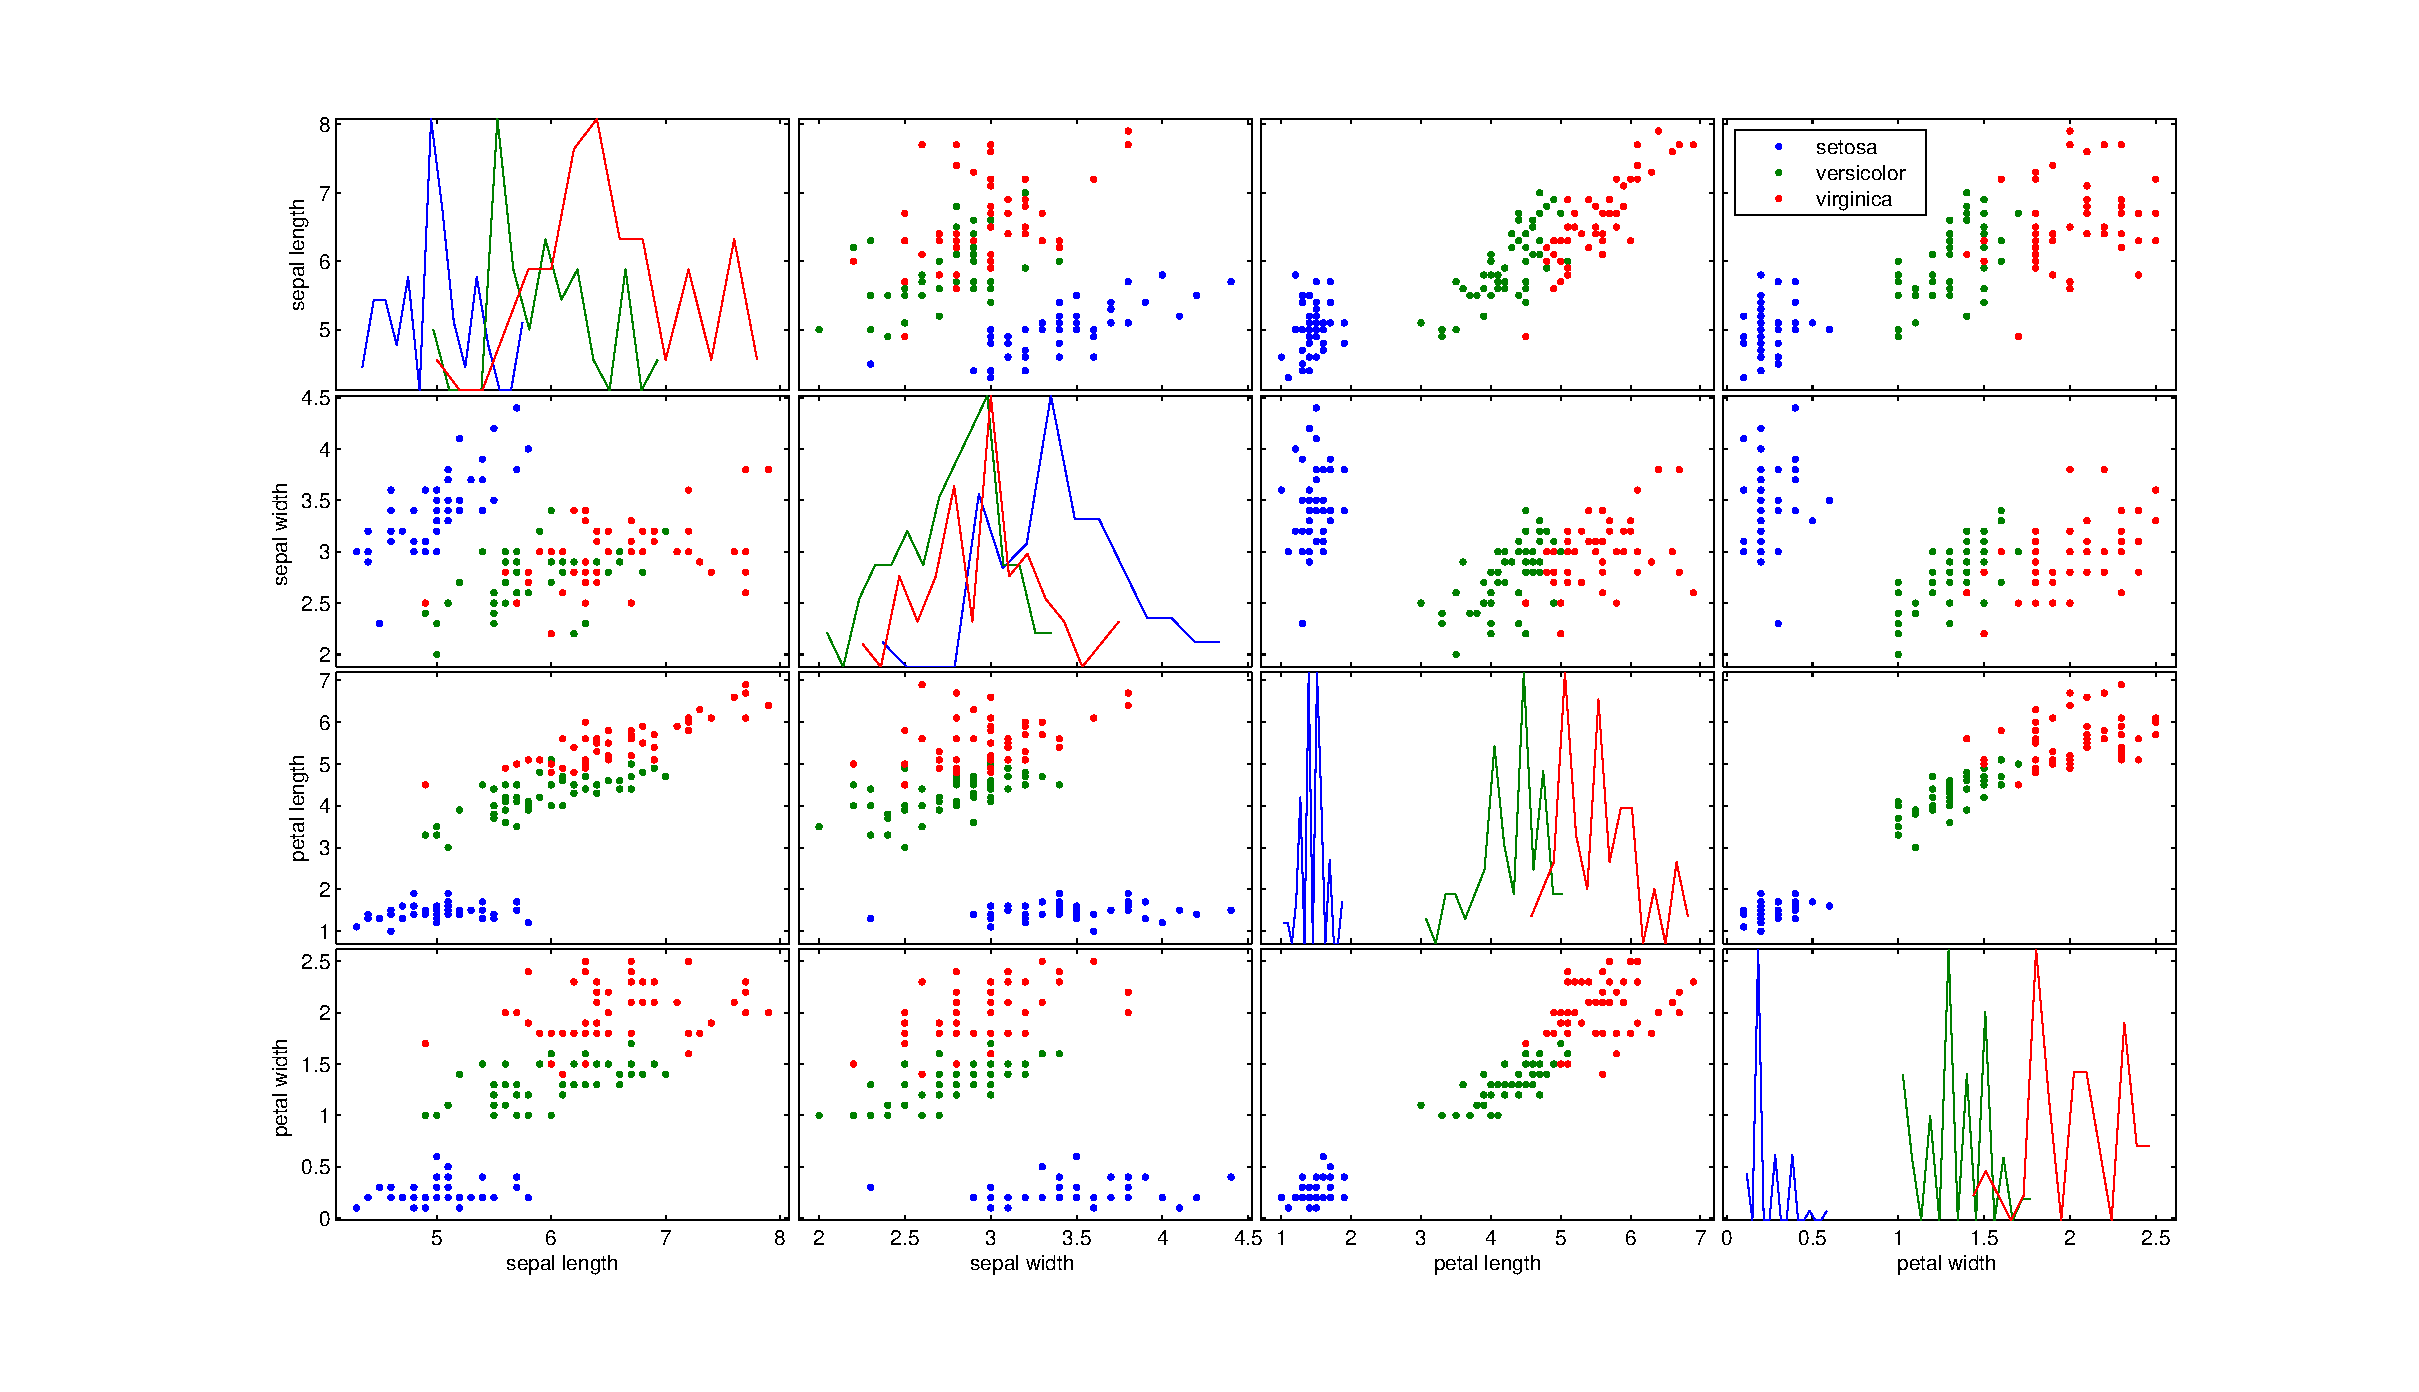
\includegraphics[width=\textwidth]{figuras/analiseIris_hist_scatterMatrix.eps}
\caption{Matriz de características.}
\label{fig:charMatrix}
\end{figure}

 Podemos perceber que a classe setosa pode facilmente ser separada das outras
 utilizando a largura ou o comprimento da pétala como variável. Nos histogramas
 localizados na parte inferior isso pode ser verificado, pétalas com
 comprimentos menores que 0,25 ou sépalas com largura menor que 0,3 de
 comprimento são claramente da classe setosa.
 Já para as duas outras características essa separação não é tão simples,
 perceba a sobreposição dos histogramas em todos os atributos bem como a mistura
 das classes nos gráficos de dispersão.
 
 \subsubsection{Base da dermatologia}
 \subsubsection{Base da coluna vertebral}



\section{Classificador de Bayes}

\subsection{Introdução}
Dada uma classificação entre M classes, o classificador de Bayes faz a seleção
de um dado $x$ com base na probabilidade de $w_i$ dado um $x$ , $P(w_i|x)$.
Assim temos:


\begin{equation}
	x \in w_i \iff P(w_i|x) \geq P(w_j|x) \forall i \neq j
\end{equation}

\subsection{Função de densidade de probabilidade}
 
\subsection{Metodologia}
\label{ss:metAplbayes}
A avaliação do classificar de Bayes foi feita de várias formas ao longo deste
trabalho, veja a subssessão \ref{ss:resultadosObtidos}. 

Na sessão \ref{ss:resultadosObtidos} são apresentados os resultados obtidos ao
aplicar o classificador de bayes utilizando como função de densidade probabilidade a Gaussiana e a
janela de parzen. Para a janela de parzen foi exibido o melhor resultado para um
determinada largura de janela do tipo gaussiana. O tamanho da janela foi
determinado após uma pesquisa linear entre valores na faixa de 0.001 e 3 para o
valor da variância.
 
\subsection{Resultados obtidos}
\label{ss:resultadosObtidos}

Na tabela \ref{tab:acuracia} são exibidos os resultados obtidos ao realizar a
classificação utilizando a regra de Bayes com funções de densidade probabilidade
(PDF) diferentes. Para cada base de dados tem-se o resultado utilizando a
Gaussiana como PDF e a janela de parzen.


\begin{table}
	\centering
    \begin{tabular}{|c|c|c|c|c|c}%
		  \multicolumn{5}{c}{Gaussiana}\\ \hline
          \hline DataSet & média & desvio Padrão & máximo & mínimo \\ \hline
          Íris & 0.974713 & 0.033802 & 1.000000 & 0.862069 \\ \hline
          Vertebra & 0.730108 & 0.052892 & 0.854839 & 0.612903 \\ \hline
          Dermatologia & 0.888584 & 0.035382 & 0.972603 & 0.821918 \\ \hline
		  
		  \multicolumn{5}{c}{Matriz de covariacia $\Sigma_i=\sigma^2I \forall
		  i$}\\
		  \hline \hline DataSet & média & desvio Padrão & máximo & mínimo \\ \hline
          Íris & 0.916092 & 0.050972 & 1.000000 & 0.793103 \\ \hline
          Vertebra & 0.698925 & 0.049818 & 0.790323 & 0.580645 \\ \hline
          Dermatologia & 0.963927 & 0.023170 & 1.000000 & 0.904110 \\ \hline 
		  
		  \multicolumn{5}{c}{Matriz de covariacia diagonal}\\ \hline
          \hline DataSet & média & desvio Padrão & máximo & mínimo \\ \hline
          Íris & 0.955172 & 0.035247 & 1.000000 & 0.862069 \\ \hline
          Vertebra & 0.787097 & 0.055776 & 0.887097 & 0.661290 \\ \hline
          Dermatologia & 0.973973 & 0.016622 & 1.000000 & 0.931507 \\ \hline     
		  
		  \multicolumn{5}{c}{Janela de Parzen}\\ \hline
          \hline DataSet & média & desvio Padrão & máximo & mínimo \\ \hline
          Íris & 0.951724 & 0.040091 & 1.000000 & 0.862069 \\ \hline
          Vertebra & 0.823656 & 0.052892 & 0.935484 & 0.693548 \\ \hline
          Dermatologia & 0.908219 & 0.026227 & 0.958904 & 0.849315
          \\ \hline
    \end{tabular}
    \caption{TTTT}
    \label{tab:acuracia}
\end{table}



\subsubsection{Busca por tamanho de janela ótima de Parzen}
\label{sss:OptSizWindSearc}

Abaixo, figura \ref{fig:parzenGraphResults} são exibidos os resultados obtidos
ao realizar a busca pelo tamanho da janela ótima de parzen para cada base de dados.
Foram considerados todos os atributos disponíveis em cada base, estes
foram normalizados e codificados apropriadamente assim como dito na
subsessão \ref{ss:normCodf}.


A linha ao centro de cada gráfico é a acurácia as outras duas são os limites.
Os limites são determinados a uma distância de um $\sigma^2$(desvio padrão)
acima e abaixo da acurácia média. Pode-se perceber que indiferentemente da base
de dados o aumento considerável da janela de parzen causa uma redução da
acurácia do classificador. Isso é causado por uma maior interferência dos vizinhos no
cálculo da probabilidade condicional o que faz com que seja levado em conta
apenas as probabilidades a priore para a determinação da classe para um dado
$x$. Isso pode ser observado quando a variância, largura da janela de parzen, é
maior que 2 na base da íris ou maior que 0.7 na base da coluna vertebral.

Os pontos máximos destas curvas nos indicam o valor ótimo da janela de parzen.
Desta forma temos na tabela \ref{tab:acuracia} o valor de acurácia e tamanho da
janela para as três bases.



\begin{figure}
	\centering
	\begin{tabular}{cc}
	  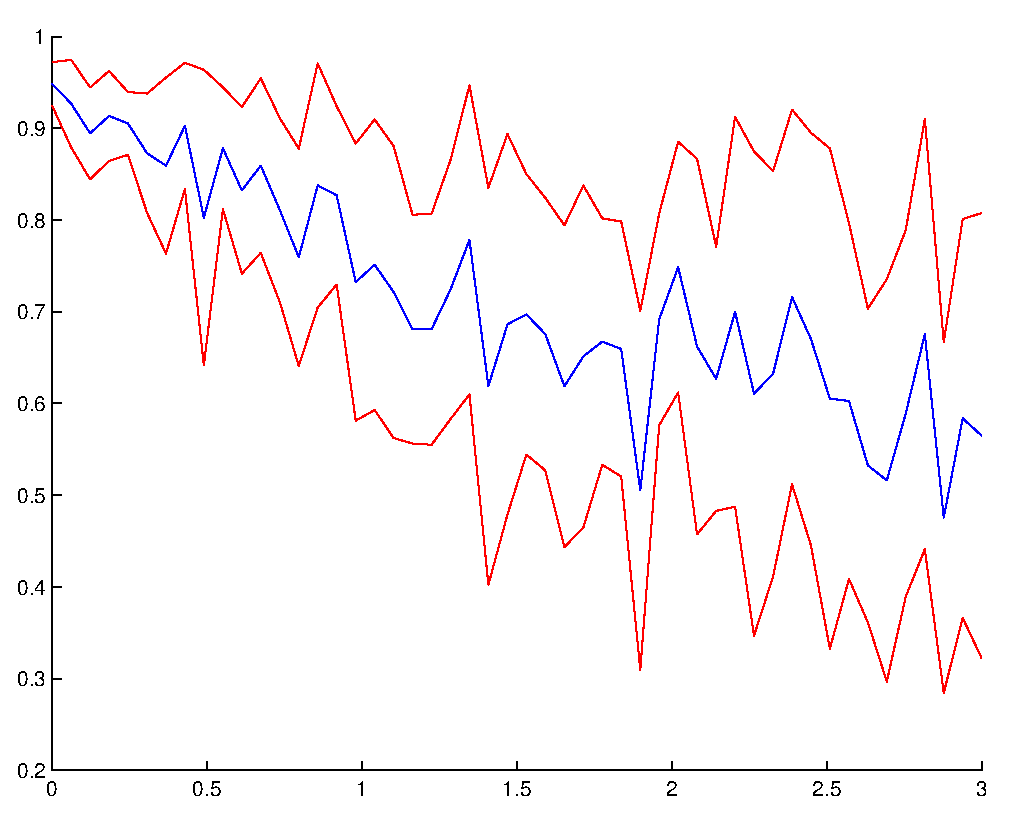
\includegraphics[width=65mm]{matlab/figura/iris_BAYES_ParzenSearch.eps} &
	  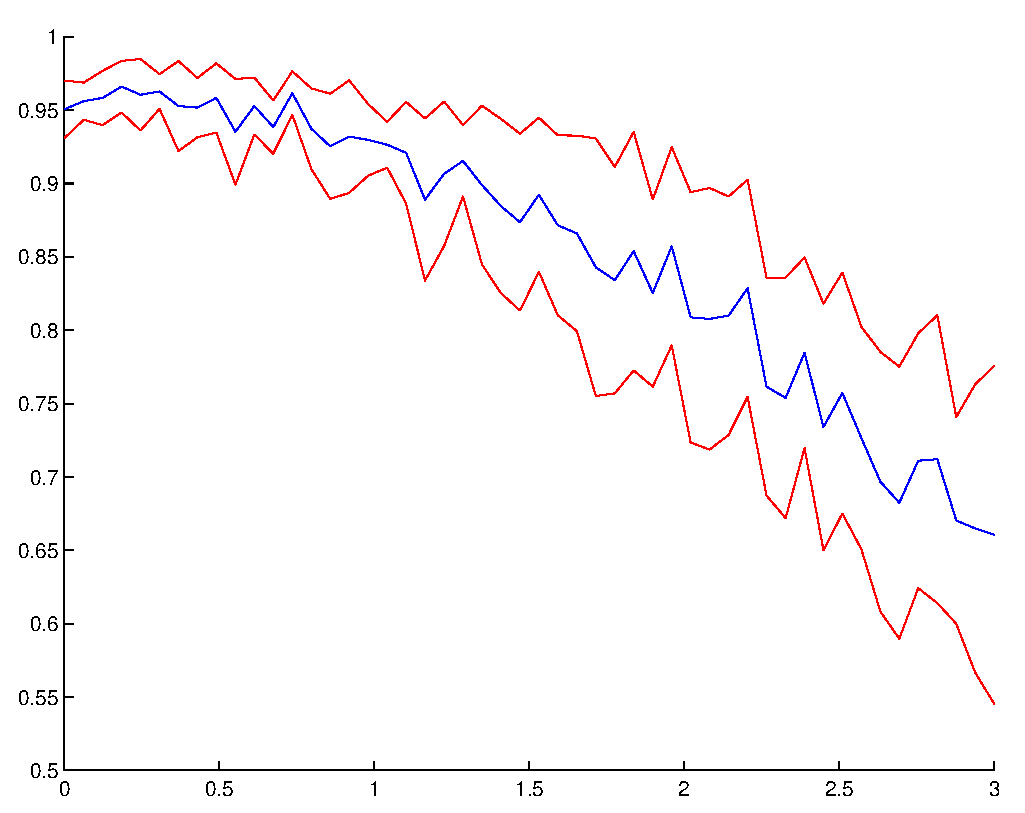
\includegraphics[width=65mm]{matlab/figura/derme_BAYES_ParzenSearch.eps}
	  \\
	(a) Íris & (b) Dermatologia \\[6pt] 
	 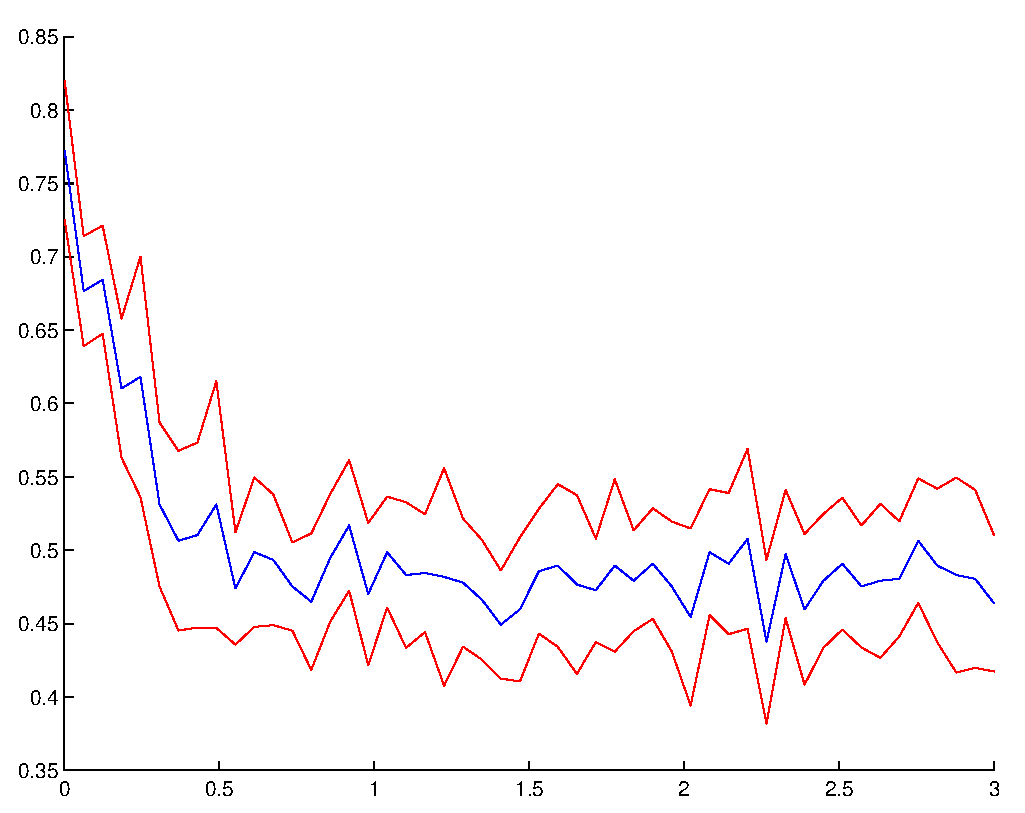
\includegraphics[width=65mm]{matlab/figura/vertebra_BAYES_ParzenSearch.eps}  &
	 \\
	 %\includegraphics[width=70mm]{matlab/figura/iris_KNN_RegDec_K75_1_3.eps} \\
	(c) Coluna Vertebral &  \\[6pt] 

	\end{tabular}

	\caption{Resultados da busca pela largura ótima da janela de parzen.}
	\label{fig:parzenGraphResults}
\end{figure}





\subsection{Análise da matriz de covariancia na definição da região de decisão}
Abaixo são apresentadas as regiões de decisões 

\subsubsection{ Matrizes de covariancia distintas. $\Sigma_i \neq \Sigma_j
\forall i \neq j $ } Com matrizes de covariancias distintas temos uma região de decisão quadrática.

\begin{figure}
	\centering
	\begin{tabular}{ccc}
	  \multicolumn{3}{c}{Íris}\\
	  %Íris
	  \includegraphics[width=40mm]{matlab/figura/gauss/iris/iris_BAYES_BayesDecP1_3_4.eps}
	  &
	  \includegraphics[width=40mm]{matlab/figura/gauss/iris/iris_BAYES_BayesDecP2_3_4.eps}
	  &
	  \includegraphics[width=40mm]{matlab/figura/gauss/iris/iris_BAYES_RegDec_3_4.eps}
	  \\
	  
	  \includegraphics[width=40mm]{matlab/figura/gauss/iris/iris_BAYES_BayesDecP1_1_4.eps}
	  &
	  \includegraphics[width=40mm]{matlab/figura/gauss/iris/iris_BAYES_BayesDecP2_1_4.eps}
	  &
	  \includegraphics[width=40mm]{matlab/figura/gauss/iris/iris_BAYES_RegDec_1_4.eps}
	  \\
	  %%-----------------------------------------------------------------------------------
	  % Dermatologia
	  \multicolumn{3}{c}{Dermatologia}\\
      \includegraphics[width=40mm]{matlab/figura/gauss/derme/derme_BAYES_BayesDecP1_1_16.eps}
      &
	  \includegraphics[width=40mm]{matlab/figura/gauss/derme/derme_BAYES_BayesDecP2_1_16.eps}
	  &
	  \includegraphics[width=40mm]{matlab/figura/gauss/derme/derme_BAYES_RegDec_1_16.eps}
	  \\	  
	  
      \includegraphics[width=40mm]{matlab/figura/gauss/derme/derme_BAYES_BayesDecP1_1_17.eps}
      &
	  \includegraphics[width=40mm]{matlab/figura/gauss/derme/derme_BAYES_BayesDecP2_1_17.eps}
	  &
	  \includegraphics[width=40mm]{matlab/figura/gauss/derme/derme_BAYES_RegDec_1_17.eps}
	  \\	
	  %%-----------------------------------------------------------------------------------
	  % Coluna
	  \multicolumn{3}{c}{Coluna Vertebral}\\
      \includegraphics[width=40mm]{matlab/figura/gauss/vertebra/vertebra_BAYES_BayesDecP1_1_2.eps}
      &
	  \includegraphics[width=40mm]{matlab/figura/gauss/vertebra/vertebra_BAYES_BayesDecP2_1_2.eps}
	  &
	  \includegraphics[width=40mm]{matlab/figura/gauss/vertebra/vertebra_BAYES_RegDec_1_2.eps}
	  \\	  
	  
      \includegraphics[width=40mm]{matlab/figura/gauss/vertebra/vertebra_BAYES_BayesDecP1_1_5.eps}
      &
	  \includegraphics[width=40mm]{matlab/figura/gauss/vertebra/vertebra_BAYES_BayesDecP2_1_5.eps}
	  &
	  \includegraphics[width=40mm]{matlab/figura/gauss/vertebra/vertebra_BAYES_RegDec_1_5.eps}
	  \\		  	  
	 \multicolumn{1}{p{40mm}}{(a) $P(W_i|x)$}
	 &
	 \multicolumn{1}{p{40mm}}{(b) Regiao de decisão}
	 &
	 \multicolumn{1}{p{40mm}}{(c) Resultado
	 da classificação dos dados sobre a regiao de decisão}
	 
	 
	\end{tabular}
	\caption{Resultados da busca pela largura ótima da janela de parzen.}

\end{figure}




\subsubsection{ Matrizes de covariancia iguais. $\Sigma_i \eq \Sigma \forall i$}

\subsubsection{Janela de Parzen}

 
\begin{figure}
	\centering
	\begin{tabular}{ccc}
	  \multicolumn{3}{c}{Íris}\\
	  %Íris
	  \includegraphics[width=40mm]{matlab/figura/parzen/iris/iris_BAYES_BayesDecP1_3_4.eps}
	  &
	  \includegraphics[width=40mm]{matlab/figura/parzen/iris/iris_BAYES_BayesDecP2_3_4.eps}
	  &
	  \includegraphics[width=40mm]{matlab/figura/parzen/iris/iris_BAYES_RegDec_3_4.eps}
	  \\
	  
	  \includegraphics[width=40mm]{matlab/figura/parzen/iris/iris_BAYES_BayesDecP1_1_4.eps}
	  &
	  \includegraphics[width=40mm]{matlab/figura/parzen/iris/iris_BAYES_BayesDecP2_1_4.eps}
	  &
	  \includegraphics[width=40mm]{matlab/figura/parzen/iris/iris_BAYES_RegDec_1_4.eps}
	  \\
	  %%-----------------------------------------------------------------------------------
	  % Dermatologia
	  \multicolumn{3}{c}{Dermatologia}\\
      \includegraphics[width=40mm]{matlab/figura/parzen/derme/derme_BAYES_BayesDecP1_1_16.eps}
      &
	  \includegraphics[width=40mm]{matlab/figura/parzen/derme/derme_BAYES_BayesDecP2_1_16.eps}
	  &
	  \includegraphics[width=40mm]{matlab/figura/parzen/derme/derme_BAYES_RegDec_1_16.eps}
	  \\	  
	  
      \includegraphics[width=40mm]{matlab/figura/parzen/derme/derme_BAYES_BayesDecP1_1_17.eps}
      &
	  \includegraphics[width=40mm]{matlab/figura/parzen/derme/derme_BAYES_BayesDecP2_1_17.eps}
	  &
	  \includegraphics[width=40mm]{matlab/figura/parzen/derme/derme_BAYES_RegDec_1_17.eps}
	  \\	
	  %%-----------------------------------------------------------------------------------
	  % Coluna
	  \multicolumn{3}{c}{Coluna Vertebral}\\
      \includegraphics[width=40mm]{matlab/figura/parzen/vertebra/vertebra_BAYES_BayesDecP1_1_2.eps}
      &
	  \includegraphics[width=40mm]{matlab/figura/parzen/vertebra/vertebra_BAYES_BayesDecP2_1_2.eps}
	  &
	  \includegraphics[width=40mm]{matlab/figura/parzen/vertebra/vertebra_BAYES_RegDec_1_2.eps}
	  \\	  
	  
      \includegraphics[width=40mm]{matlab/figura/parzen/vertebra/vertebra_BAYES_BayesDecP1_1_5.eps}
      &
	  \includegraphics[width=40mm]{matlab/figura/parzen/vertebra/vertebra_BAYES_BayesDecP2_1_5.eps}
	  &
	  \includegraphics[width=40mm]{matlab/figura/parzen/vertebra/vertebra_BAYES_RegDec_1_5.eps}
	  \\		  	  
	 \multicolumn{1}{p{40mm}}{(a) $P(W_i|x)$}
	 &
	 \multicolumn{1}{p{40mm}}{(b) Regiao de decisão}
	 &
	 \multicolumn{1}{p{40mm}}{(c) Resultado
	 da classificação dos dados sobre a regiao de decisão}
	 
	 
	\end{tabular}
	\caption{Região de decisão calculada utilizando janela de parzen com largura
	$\sigma^2=0.05I$ .}

\end{figure}

\subsubsection{Região de decisão}

\subsubsection{Matriz Confusão}
Na tabela \ref{tab:confMatKNN} é exibida a matriz confusão obtida para K igual a
10. Esse valor de k foi escolhido devido aos testes de acurácia em
função de k mostrarem que com este valor é obtida a melhor acurácia. Além da
matriz confusão  a tabela \ref{tab:knnAnalis} traz os
resultados, falso-positivo, falso-negativo, verdadeiro-positivo e
verdadeiro-negativo. 


\section{Segmentação uitlizando Classificador de Bayes}
 A segmentação de uma imagem é realizada levando em
consideração a intensidade dos pixels nas três componentes RGB.
A definição dos dados de de uma classe é feita a partir da seleção de $k$
regiões da imagem, não necessariamente de mesma área $A_i$. A área é utilizada
para calcular a probabilidade a priore por isso classes com uma diferença de
área muito grande podem impactar na classificação.
Assim temos:

\begin{equation}
	P(w_i) =  \frac{A_i}{\sum_{i=1}^{k}{A_J}}
\end{equation}

\subsection{PDF Gaussiana}
Nas figuras \ref{fig:resultBandSegParadise} e \ref{fig:resultGaussSegParadise}
são apresentado o resultado da segmentação de duas imagens utilizando o
classificador Bayessiano. Os parâmetros $\sigma^2$ e $\mu$ são estimados de
acordo com os dados de cada classe individualmente. Assim temos na figuras
\ref{fig:resultBandSegParadise} e \ref{fig:resultGaussSegParadise} o resultado
deste classificador sobre 2 imagens distintas.

\begin{figure}
	\centering
	\begin{tabular}{ccc}
	\multicolumn{3}{c}{
	  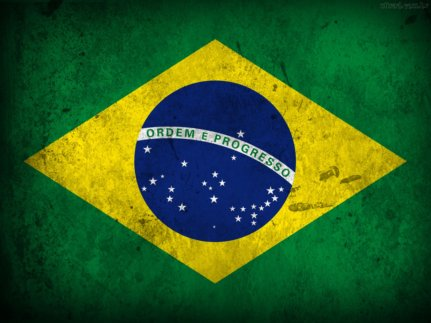
\includegraphics[width=45mm]{matlab/figura/gauss/segmentacao/brasil.jpg} 
	  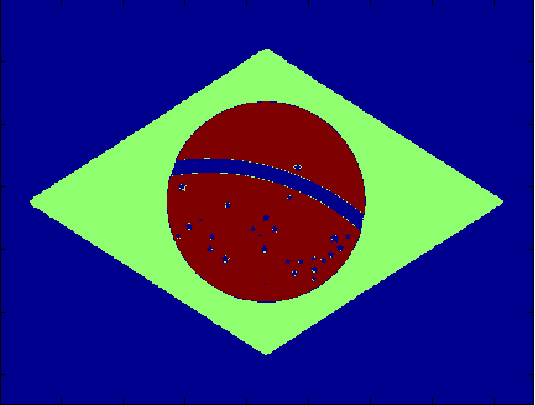
\includegraphics[width=45mm]{matlab/figura/gauss/segmentacao/brasilSeg.png}
	  }\\ 
	\multicolumn{3}{c}{
	 \hspace{1cm} (a) Original \hspace{15mm} (b)Resultado da Segmentação
	  }\\ 	  
	 
\includegraphics[width=30mm]{matlab/figura/gauss/segmentacao/bc1.png}&   
	 
\includegraphics[width=30mm]{matlab/figura/gauss/segmentacao/bc2.png}& 
	 
\includegraphics[width=30mm]{matlab/figura/gauss/segmentacao/bc3.png} \\
	(c) $A_1$ & (d) $A_2$ & (e) $A_3$\\[6pt] 

	\end{tabular}
	\caption{Resultado da segmentação utilizando o classificador Bayessiano. Na
	linha inferior são apresentados as amostras utilizadas para definir as
	classes. As áreas utilizadas são:(c) céu, (d) areia e (e) coqueiro}
	\label{fig:resultBandSegParadise}
\end{figure}


\begin{figure}
	\centering
	\begin{tabular}{ccc}
	\multicolumn{3}{c}{
	  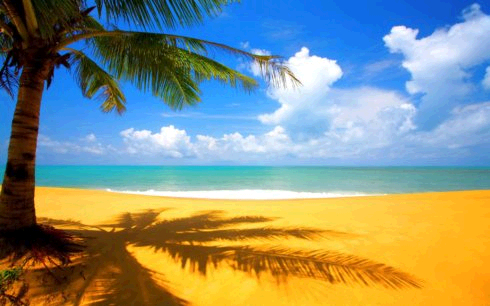
\includegraphics[width=45mm]{matlab/figura/gauss/segmentacao/paradise.jpg} 
	  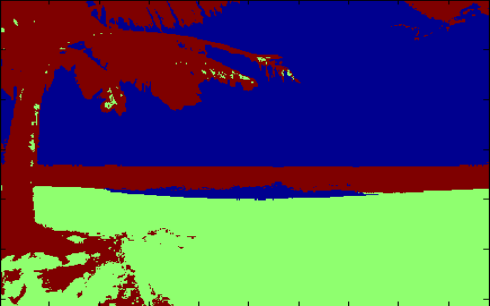
\includegraphics[width=45mm]{matlab/figura/gauss/segmentacao/paradiseRes.png}
	  }\\ 
	\multicolumn{3}{c}{
	 \hspace{1cm} (a) Original \hspace{15mm} (b)Resultado da Segmentação
	  }\\ 	  
	 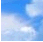
\includegraphics[width=30mm]{matlab/figura/gauss/segmentacao/pc1.png}&   
	 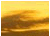
\includegraphics[width=30mm]{matlab/figura/gauss/segmentacao/pc2.png}& 
	 \includegraphics[width=30mm]{matlab/figura/gauss/segmentacao/pc3.png} \\
	(c) $A_1$ & (d) $A_2$ & (e) $A_3$\\[6pt] 

	\end{tabular}
	\caption{Resultado da segmentação utilizando o classificador Bayessiano. Na
	linha inferior são apresentados as amostras utilizadas para definir as
	classes. As áreas utilizadas são:(c) céu, (d) areia e (e) coqueiro}
	\label{fig:resultGaussSegParadise}
\end{figure}



\subsection{PDF Janela de Parzen}
Abaixo é apresentado o resultado da segmentação de uma imagem utilizando o
classificador Bayessiano, desta vez utilizando janela de parzen como função de
densidade probabilidade. Foram realizados três testes com três variancias da
janela, valor de h, distintas. Os valores testados foram, 0.05, 0.5 e 1. Com o
aumento do valor de h houve uma maior suavização


\begin{figure}
	\centering
	\begin{tabular}{cc}
	  \includegraphics[width=45mm]{matlab/figura/gauss/segmentacao/paradise.jpg} & 
	  \includegraphics[width=45mm]{matlab/figura/parzen/segmentacao/paradiseRes.png}
	  \\ 
	  (a) Original & (b) h=0.05\\
	  \includegraphics[width=45mm]{matlab/figura/parzen/segmentacao/paradiseRes05.png} & 
	  \includegraphics[width=45mm]{matlab/figura/parzen/segmentacao/paradiseRes1.png}
	   \\
	  (c) h=0.5 & (d) h=1\\
	\end{tabular}
	\caption{Resultado da segmentação utilizando o classificador Bayessiano com
	janela de parzen.
	Com o aumento do valor de h pode-se notar que a segmentação se torna mais
	suave.}
	\label{fig:resultGaussSegParadise}
\end{figure}



\bookmarksetup{startatroot}% 
% ---

% ---
% Conclusão
% ---
\section*{Considerações finais}




\addcontentsline{toc}{section}{Considerações finais}



% ----------------------------------------------------------
% ELEMENTOS PÓS-TEXTUAIS
% ----------------------------------------------------------
\postextual

% ----------------------------------------------------------
% Referências bibliográficas
% ----------------------------------------------------------
\bibliography{bib,iris}

% ----------------------------------------------------------
% Glossário
% ------------------------------------ ----------------------
%
% Há diversas soluções prontas para glossário em LaTeX. 
% Consulte o manual do abnTeX2 para obter sugestões.
% 
%\glossary 

% ----------------------------------------------------------
% Apêndices
% ----------------------------------------------------------


\end{document}